\documentclass[../main/main]{subfiles}
\setcounter{chapter}{0}% Chapter番号-1の値を設定する
\begin{document}
\chapter{テンプレートの使い方}
\section{概要}
本テンプレートは,卒論用の\LaTeX テンプレートである.
適宜書き換えて使用すること.
最新版は,
\url{https://github.com/takala4/Thesis_Template}
にある.
\par
各ファイルを個別にコンパイルすることもできるが,\verb|main/main.tex|をコンパイルすることで,全てのファイルをコンパイルすることもできる.
\par
パッケージの追加やオリジナルコマンドの定義は,\verb|main/main.tex|に記述する.ここに記述することで,各ファイルに一括で適用される.
\par
新しいサブファイルを追加する場合は,main.texに\verb|\subfile{ファイル名}|を追加する.


\newpage
\section{overleafでの使用方法}\label{sec:1_overleaf}
overleafで使用することもできる.設定のポイントは次の3点.
\paragraph{ポイント1:基本設定}
\begin{itemize}
  \item Compiler: \verb|LaTeX|
  \item Main document: \verb|Thesis/main/main.tex|
  \item その他:基本的にデフォルトで可
\end{itemize}
\paragraph{ポイント2:latexmkrcの設置}
その他,\verb|latexmkrc|ファイル(拡張子はなし)を用意する.
以下を記載し,最上位階層に配置する.
\begin{lstlisting}
    $latex = 'uplatex';
    $bibtex = 'bibtex';
    $dvipdf = 'dvipdfmx %O -o %D %S';
    $makeindex = 'mendex -U %O -o %D %S';
    $pdf_mode = 3;
    $ENV{'BIBINPUTS'}='..//input//:' . $ENV{'BIBINPUTS'};
\end{lstlisting}
\paragraph{ポイント3:bibファイルの参照設定}
\verb|main.tex|の\verb|\addbibresource{../input/refs.bib}|を\verb|\addbibresource{refs.bib}|に変更する.
ただし,bibファイルの配置場所は,\verb|../input/refs.bib|のままである.
\begin{lstlisting}[language={[latex]TeX}]
  \addbibresource{refs.bib} %bibファイル (for overleaf)
  % \addbibresource{../input/refs.bib} %bibファイル (for local compile)
\end{lstlisting}



\newpage
\section{ファイル構成}
ディレクトリ構成は次の通り.頭に数字がついているのは,ファイルエクスプローラー上で,ディレクトリが綺麗に並ぶようにするためである.ややこしい場合は適宜改変してよい.ただし,\verb|main/main.tex|に相当するディレクトリとファイルに関しては,アンダーライン\verb|_|を使うことができない.
\begin{framed}
  \dirtree{%
  .1 Thesis/.
  .2 000\_cover/.
  .3 000\_cover.tex [表紙].
  .2 001\_abstract/.
  .3 001\_abstract.tex [要旨].
  .2 01\_chap/.
  .3 01\_chap.tex [第1章].
  .3 image/.
  .4 sample.pdf.
  .2 02\_chap/.
  .3 02\_chap.tex [第2章].
  .2 03\_chap/.
  .3 03\_chap.tex [第3章].
  .2 98\_appendix/.
  .3 98\_appendix.tex [付録].
  .2 99\_thank/.
  .3 99\_thank.tex [謝辞].
  .2 main/.
  .3 main.tex [全体].
  .2 input/.
  .3 takalastyle.sty.
  .3 refs.bib.
  }
\end{framed}


\newpage
\section{参考文献}
参考文献の管理はbibを用いて行う.
\subsection{bibファイル}
bibファイルは\verb|input/refs.bib|に保存する.
\par
bibファイルの各文献は,Google Scholarで引用した文献をBibTeX形式で出力することで簡単に作成できる.
まず,Google Scholarで引用したい文献を検索し,「引用」を選択する.
\begin{figure}[!ht]
  \centering
  
\includegraphics[clip, width=0.5\columnwidth]{image/bib1.png}
  \label{fig:bib1}
\end{figure}
\par
次に「BibTeX」を選択する.
\begin{figure}[!ht]
  \centering
  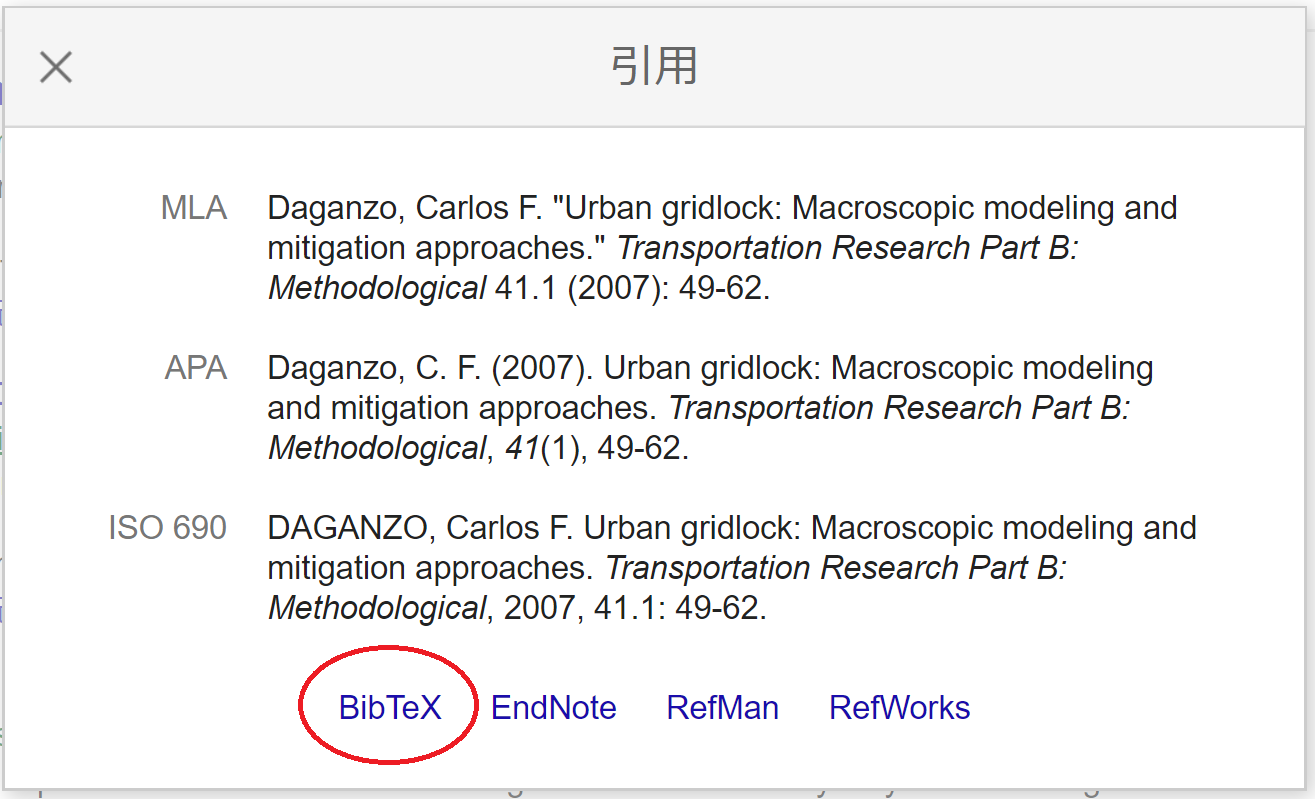
\includegraphics[clip, width=0.5\columnwidth]{image/bib2.png}
  \label{fig:bib1}
\end{figure}
\par
すると,以下のようなコードが記述された別ページに遷移する.
\begin{figure}[!ht]
  \centering
  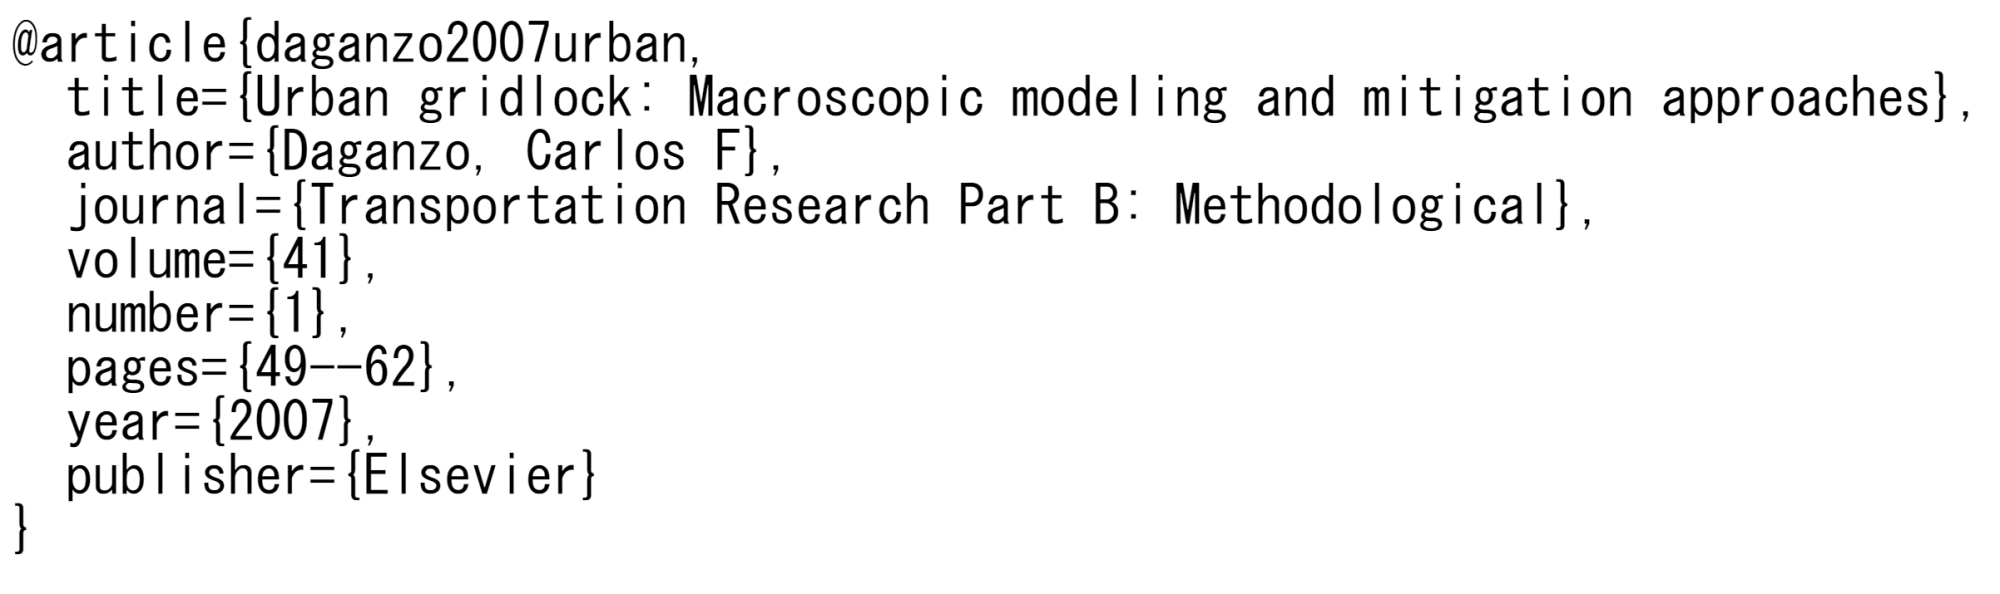
\includegraphics[clip, width=0.5\columnwidth]{image/bib3.png}
  \label{fig:bib1}
\end{figure}
\par
これをコピーして,refs.bibに貼り付ける.

\subsection{日本語文献}\label{subsec:japanese_bib}
日本語文献を扱う場合のbibデータの注意点は以下である:
\begin{itemize}
  \item keyは必ず半角英数字にする.
  \item langidという新しいフィールドを追加しjapaneseと設定する.
  \item 姓名の区切りは半角カンマとする.
\end{itemize}
つまり,次のように記述すれば良い.
  \begin{lstlisting}[language={[latex]TeX}]
    @article{TAKAYAMA2014DEVELOPMENT,
    title= {新経済地理学に基づく空間応用一般均衡モデルの開発},
    author= {高山,雄貴 and 赤松,隆 and 石倉,智樹},
    journal= {土木学会論文集 D3 (土木計画学)},
    volume={70},
    number={4},
    pages={245--258},
    year={2014},
    publisher={公益社団法人 土木学会},
    langid={japanese}
  }
  \end{lstlisting}
このようにしない場合,日本語文献が適切に処理されない.

\subsection{本文内での引用}
本文内での引用は\verb|\cite{キー}|を用いて行う.
例えば,\verb|\citet{Vickrey1969-ic}|と記述すると,\citet{Vickrey1969-ic}となる.
その他,\verb|\citep|,\verb|\citeauthor|,\verb|\citeyear|などがある.
詳しくは,\url{https://www.overleaf.com/learn/latex/Natbib\_citation\_styles}を参照のこと.
  \begin{itemize}
    \item \verb|\citet{キー}|:著者名を引用する.例:\citet{Vickrey1969-ic}
    \item \verb|\citep{キー}|:括弧付きで引用する.例:\citep{Vickrey1969-ic}
    \item \verb|\citeauthor{キー}|:著者名のみを引用する.例:\citeauthor{Vickrey1969-ic}
    \item \verb|\citeyear{キー}|:年のみを引用する.例:\citeyear{Vickrey1969-ic}
    \item \verb|\cite{キー}|:著者名と年を引用する.例:\cite{Vickrey1969-ic}
  \end{itemize}
 なお,3人以上の著者の場合,英語文献の場合,firstauthor et al.となる.日本語文献の場合,firstauthorらとなる.
\begin{itemize}
  \item 著者2人(英語):\citet{arnott2011corridor}
  \item 著者3人以上(英語):\citet{arnott1990economics}
  \item 著者2人(日本語):\citet{TAKAYAMA2011SPATIAL}
  \item 著者3人以上(日本語):\citet{TAKAYAMA2014DEVELOPMENT}
\end{itemize}


\subsection{文献管理ツール}
Google Scholarで一つずつ文献を引用するのは面倒である.
世の中には様々な文献管理ツールがあり,これらを用いることで簡単に文献を管理することができる.
また,一括でbibファイルを出力することもできる.
\begin{itemize}
  \item Paperpile
  \item JabRef
  \item Mendeley
  \item Zotero
  \item EndNote
  \item Citavi
\end{itemize}
おすすめは,Paperpileであるが,月2.99ドルかかる.

\newpage
\section{図の挿入}
図はpng, pdf, eps, jpgなどの画像ファイルを用いて挿入する.pdfがおすすめ.
\par
図の挿入は,figure環境を用いて行う.
\begin{lstlisting}[language={[latex]TeX}]
  \begin{figure}[!ht]
    \center
    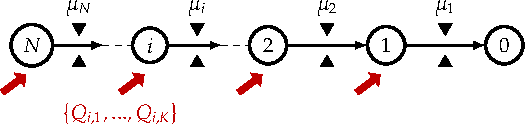
\includegraphics[clip, width=0.5\columnwidth]{image/sample.pdf}
    \caption{$N$個の起点からなるコリドーネットワーク}
    \label{fig:CorridorNetwork}
  \end{figure}
\end{lstlisting}

\begin{figure}[!ht]
  \center
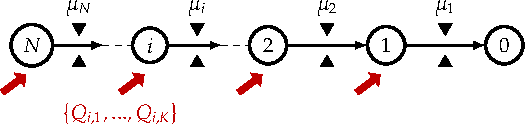
\includegraphics[clip, width=0.5\columnwidth]{image/sample.pdf}
  \caption{$N$個の起点からなるコリドーネットワーク}
  \label{fig:CorridorNetwork}
\end{figure}

\newpage
\section{表の挿入}
表は作成は次のように記述する.
\begin{lstlisting}[language={[latex]TeX}]
  \begin{table}[ht]
    \centering % 表を中央揃えにする
    \caption{サンプルテーブル} % 表のタイトル
    \label{tab:sample_table} % 表を参照するためのラベル
    \begin{tabular}{lcr} % 列の配置: left, center, right
    \toprule % 上部の罫線
    列1のヘッダ & 列2のヘッダ & 列3のヘッダ \\
    \midrule % 中間の罫線
    行1のデータ1 & 行1のデータ2 & 行1のデータ3 \\
    行2のデータ1 & 行2のデータ2 & 行2のデータ3 \\
    行3のデータ1 & 行3のデータ2 & 行3のデータ3 \\
    \bottomrule % 下部の罫線
   \end{tabular}
  \end{table}
\end{lstlisting}
これをコンパイルすると,次のようになる.
\begin{table}[ht]
  \centering % 表を中央揃えにする
  \caption{サンプルテーブル} % 表のタイトル
  \label{tab:sample_table} % 表を参照するためのラベル
  \begin{tabular}{lcr} % 列の配置: left, center, right
  \toprule % 上部の罫線
  列1のヘッダ & 列2のヘッダ & 列3のヘッダ \\
  \midrule % 中間の罫線
  行1のデータ1 & 行1のデータ2 & 行1のデータ3 \\
  行2のデータ1 & 行2のデータ2 & 行2のデータ3 \\
  行3のデータ1 & 行3のデータ2 & 行3のデータ3 \\
  \bottomrule % 下部の罫線
 \end{tabular}
\end{table}

\newpage
\section{数式}
数式は,align環境を用いて記述すると良い.
\begin{lstlisting}[language={[latex]TeX}]
\begin{align}
  &y = a x^{2} + bx + c
  \\
  &\VtA = 
  \begin{bmatrix}
    1 & 2 & 3 \\
    4 & 5 & 6 \\
    7 & 8 & 9
  \end{bmatrix}
  \\
  &\begin{dcases}
    F(x) = 0 &\text{if}   \quad x>0
    \\
    F(x) \geq 0 &\text{if} \quad x=0
  \end{dcases}
\end{align}
\end{lstlisting}
\begin{align}
  &y = a x^{2} + bx + c
  \\
  &\VtA = 
  \begin{bmatrix}
    1 & 2 & 3 \\
    4 & 5 & 6 \\
    7 & 8 & 9
  \end{bmatrix}
  \\
  &\begin{dcases}
    F(x) = 0 &\text{if}   \quad x>0
    \\
    F(x) \geq 0 &\text{if} \quad x=0
  \end{dcases}
\end{align}

\newpage
\section{定理環境}
定義,仮定,定理,命題,補題,系などは,\verb|amsthm|パッケージを用いて記述する.
\begin{itemize}
  \item 定義:\verb|\begin{dfn}\text{~}\end{dfn}|
  \item 仮定:\verb|\begin{asm}\text{~}\end{asm}|
  \item 命題:\verb|\begin{pro}\text{~}\end{pro}|
  \item 定理:\verb|\begin{thm}\text{~}\end{thm}|
  \item 補題:\verb|\begin{lem}\text{~}\end{lem}|
\end{itemize}
\begin{lstlisting}[language={[latex]TeX}]
  \begin{dfn}[凸集合]
    集合 $\ClS \subset \mathbb{R}^n$ が凸集合であるとは,
    任意の $x, y \in \ClS$ と任意の $\lambda \in [0, 1]$ に対して,
    $\lambda x + (1 - \lambda) y \in \ClS$ が成り立つことをいう.
  \end{dfn}
  \begin{thm}[角谷の不動点定理]
    \label{thm:Kakutani}
    \$S$ を,ユークリッド空間 $\mathbb{R}^n$ の空でない
    コンパクト凸部分集合とする.
    $\varphi: S \rightarrow 2^S$ を $S$ 上の集合値関数で,
    閉グラフと次の性質を備えるものとする:
    $\varphi(x)$ は $x \in S$ に対して空でない凸集合である.
    このとき,$\varphi$ は不動点を持つ.
  \end{thm}
\end{lstlisting}
\begin{dfn}[凸集合]
  集合 $\ClS \subset \mathbb{R}^n$ が凸集合であるとは,任意の $x, y \in \ClS$ と任意の $\lambda \in [0, 1]$ に対して,$\lambda x + (1 - \lambda) y \in \ClS$ が成り立つことをいう.
\end{dfn}
\begin{thm}[角谷の不動点定理]
  \label{thm:Kakutani}
  $S$ を,ユークリッド空間 $\mathbb{R}^n$ の空でないコンパクト凸部分集合とする.$\varphi: S \rightarrow 2^S$ を $S$ 上の集合値関数で,閉グラフと次の性質を備えるものとする:$\varphi(x)$ は $x \in S$ に対して空でない凸集合である.
  このとき,$\varphi$ は不動点を持つ.
\end{thm}



\newpage
\section{アルゴリズム}
アルゴリズム(疑似コード)は,algorithm, algpseudocodeパッケージを用いて記述する.詳しい使い方は,\url{https://www.overleaf.com/learn/latex/algorithms}を参照のこと.
\begin{lstlisting}[language={[latex]TeX}]
  \begin{algorithm}[ht]
    \caption{サンプルアルゴリズム}
    \label{alg:sample_algorithm}
    \begin{algorithmic}[1]
      \Require $x$,$y$
      \Ensure $z$
      \State $z \gets x + y$
      \State \Return $z$
    \end{algorithmic}
  \end{algorithm}
\end{lstlisting}
\begin{algorithm}[!ht]
  \caption{サンプルアルゴリズム}
  \label{alg:sample_algorithm}
  \begin{algorithmic}[1]
    \Require $x$,$y$
    \Ensure $z$
    \State $z \gets x + y$
    \State \Return $z$
  \end{algorithmic}
\end{algorithm}


\newpage
\section{数式,図表,命題等の引用}
\verb|\label{ラベル名}|を用いて,数式,図表,命題等にラベルを付ける.
\verb|\cref{ラベル名}|を用いて,数式,図表,命題等を参照する.
\begin{lstlisting}[language={[latex]TeX}]
  \begin{align}
    &y = a x^{2} + bx + c
    \label{eq:sample_equation}
  \end{align}
  \cref{eq:sample_equation}は,二次関数である.
\end{lstlisting}
\begin{align}
  &y = a x^{2} + bx + c
  \label{eq:sample_equation}
\end{align}
\cref{eq:sample_equation}は,二次関数である.

\newpage
\section{付録の挿入}
2種類の方法がある.
\subsection{各chapterごとに付録を挿入する場合}
付録は,subappendices環境を用いて挿入する.
\begin{lstlisting}[language={[latex]TeX}]
  \begin{subappendices}
    \section{証明}
    ここは章ごとの付録.
  \end{subappendices}
\end{lstlisting}

\subsection{論文の最後に付録を挿入する場合}
付録は,appendix環境を用いて挿入する.
各chapterと同じように,subfileを作成する.
ただし,次のようにchapterの前に\verb|\appendix|を挿入する.
\begin{lstlisting}[language={[latex]TeX}]
  
  \begin{document}
  \appendix
  \chapter{定理Iの証明}
    ここは付録.

  \chapter{定理IIの証明}
    ここは付録.

  \bibdummy{1}
  \end{document}

\end{lstlisting}



\begin{subappendices}
  \section{証明}
  ここは章ごとの付録.
\end{subappendices}

\bibdummy{1}% {1}にするとsubfileごとのコンパイルでも参考文献を出力する.{0}にすると出力しない.
\end{document}
